\section{Results and Discussion} \label{sec:results}

Preliminary experiments within a bounded 2D CA domain for 1,000 update steps, using learned rule sets reported in work on differentiable Lenia
\citep{hamon2022learning}.
Example runs shown were generated with the \texttt{crea1} rule set, which exhibited occasional self-catalyzed replication events.
Notebook code at \url{https://hopth.ru/ev} also includes examples from an alternate \texttt{crea2} ruleset producing non-replicator solitons.

\begin{figure}[htbp]
  \centering
  % Top row: Sparse images
  \begin{subfigure}[b]{0.65\textwidth}
    \centering
    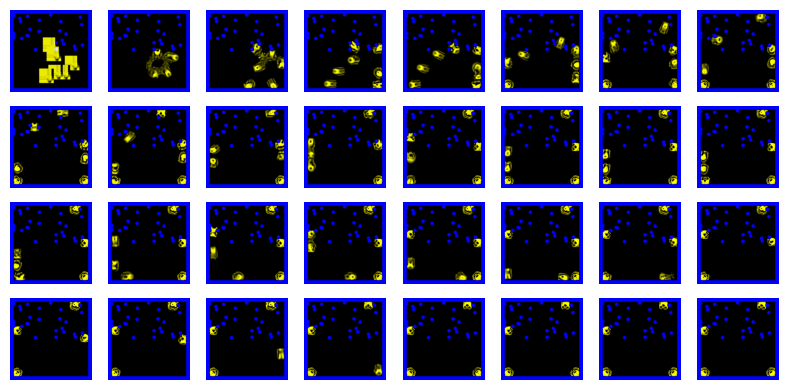
\includegraphics[width=\textwidth]{img/dev-timelapse-sparse.png}
    \caption{Sparse timelapse}
    \label{fig:dev-sample:dev-timelapse-sparse}
  \end{subfigure}%
  \hfill
  \begin{subfigure}[b]{0.35\textwidth}
    \centering
    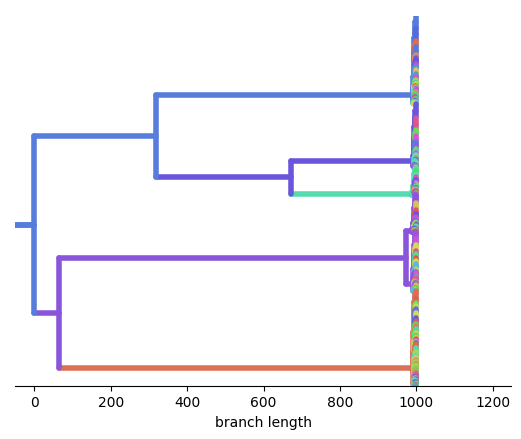
\includegraphics[width=\textwidth]{img/dev-phylo-sparse.png}
    \caption{Sparse phylo}
    \label{fig:dev-sample:dev-phylo-sparse}
  \end{subfigure}

  \vspace{1em}

  % Bottom row: Dense images
  \begin{subfigure}[b]{0.65\textwidth}
    \centering
    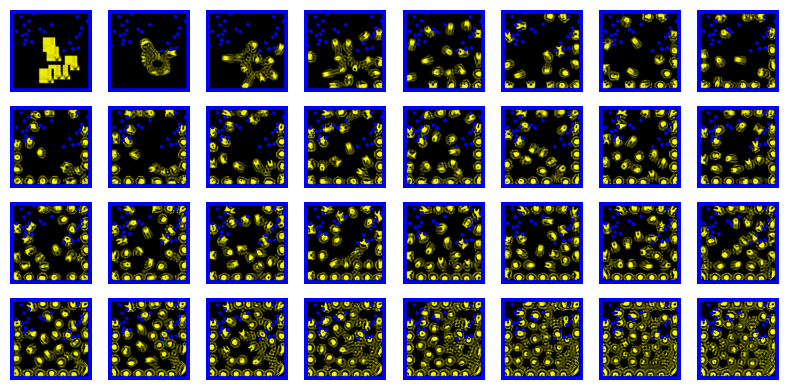
\includegraphics[width=\textwidth]{img/dev-timelapse-dense.png}
    \caption{Dense timelapse}
    \label{fig:dev-sample:dev-timelapse-dense}
  \end{subfigure}%
  \hfill
  \begin{subfigure}[b]{0.35\textwidth}
    \centering
    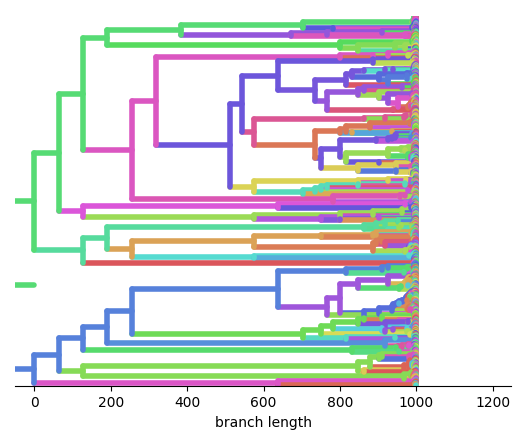
\includegraphics[width=\textwidth]{img/dev-phylo-dense.png}
    \caption{Dense phylo}
    \label{fig:dev-sample:dev-phylo-dense}
  \end{subfigure}

  \caption{Sample results using naive local max attribution rule with differentiable Lenia \citep{hamon2022learning}.
  Top row: sparse simulation outcome; note the soliton-pair autocatalytic replication event in the bottom right corner.
  Bottom row: dense simulation outcome.
  The sparse animation is available at \url{https://hopth.ru/et} and the dense animation at \url{https://hopth.ru/eu}.
  Source notebook is at \url{https://hopth.ru/ev}.
}
  \label{fig:dev-sample}
\end{figure}


Figure \ref{fig:dev-sample} compares example Lenia time-lapses with corresponding phylogenies reconstructed from all CA cells with end-state activation above a fixed threshold.
Obstacle layout (blue circles) was generated randomly, and differs between examples.
In the first example, several soliton evaporation events occur along with a small amount of replicator activity, yielding a sparse population size.
In the second example, intense soliton replication occurs near the beginning of the simulation, leading the CA space to be mostly filled.

Phylogenies were reconstructed from 64-bit hstrat/dstream annotations, curated according to the tilted retention policy.
Annotations were propagated using a naive argmax attribution function, described in Section \ref{sec:attribution}.
